%======================================================================
\NEWMOD
%======================================================================

\section{\sCODE}

%----------------------------------------------------------------------

\logo{\hfill\hyperlink{outline<1>}{\icon}}

\begin{frame}[fragile,label=s-CODE] 
\modframetitle{\sCODE}
\scriptsize
\begin{center}
\begin{minipage}{3.25in}
\begin{enumerate}
\item \hyperlink{ss-oop<1>}   {\BUTTON {\ssOop}}
\item \hyperlink{ss-components<1>}   {\BUTTON {\ssComponents}}
\item \hyperlink{ss-classes<1>}   {\BUTTON {\ssClasses}}
\item \hyperlink{ss-classes-org<1>}   {\BUTTON {\ssClasses-org}}
\item \hyperlink{ss-problems<1>}   {\BUTTON {\ssProblems}}
\item \hyperlink{ss-data<1>}   {\BUTTON {\ssData}}
\item \hyperlink{ss-fields<1>}   {\BUTTON {\ssFields}}
\item \hyperlink{ss-particles<1>}   {\BUTTON {\ssParticles}}
\item \hyperlink{ss-boundary<1>}   {\BUTTON {\ssBoundary}}
\item \hyperlink{ss-initial<1>}   {\BUTTON {\ssInitial}}
\item \hyperlink{ss-refine<1>}   {\BUTTON {\ssRefine}}
\item \hyperlink{ss-stopping<1>}   {\BUTTON {\ssStopping}}
\item \hyperlink{ss-methods<1>}   {\BUTTON {\ssMethods}}
\item \hyperlink{ss-control<1>}   {\BUTTON {\ssControl}}
\item \hyperlink{ss-amr<1>}   {\BUTTON {\ssAmr}}
\item \hyperlink{ss-exchange<1>}   {\BUTTON {\ssExchange}}
\end{enumerate}
\end{minipage}
\end{center}
\end{frame}

\logo{\hfill\hyperlink{s-CODE<1>}{\icon}}

%======================================================================
\NEWSEC
%======================================================================

\subsection{\ssOop}

\begin{frame}[fragile,label=ss-oop] 
\secframetitle{\ssOop}
\bluebf{Enzo-P/Cello's design is \blueit{object-oriented}}

\begin{itemize}
\item Package-level design
\begin{itemize}
\item \bluecode{Enzo-P} \bluetext{application} implemented using \greencode{Cello} \greentext{AMR framework}
\item \greencode{Cello} implemented using \redcode{Charm++} \redtext{parallel programming system}
\end{itemize}
\item Component-level design
\begin{itemize}
\item \code{Cello} is decomposed into high-level \greenit{components}
\item Components are comprised of one or more \greenit{classes}
\end{itemize}
\item Source code is organized by package, component, and class
\begin{itemize}
\footnotesize
\item \bluecode{Enzo-P}:
\bluecode{cello-src/src/Enzo/}\blueit{enzo\_<class>}\bluecode{.[ch]pp}
\item \greentext{Cello}:
\greencode{cello-src/src/Cello/}\greenit{<component>\_<class>}\greencode{.[ch]pp}
\end{itemize}
\end{itemize}

\end{frame}

%----------------------------------------------------------------------

%\begin{frame}[fragile] 
%\secframetitle{\ssOop}
%\end{frame}
 % How is object-oriented programming used in Enzo-P?
%======================================================================
\NEWSEC
%======================================================================

\subsection{\ssComponents}

%----------------------------------------------------------------------

\begin{frame}[fragile,label=ss-components] 
\secframetitle{\ssOop}
\framesubtitle{Cello software components}
\vspace{-0.2in}
\begin{center}
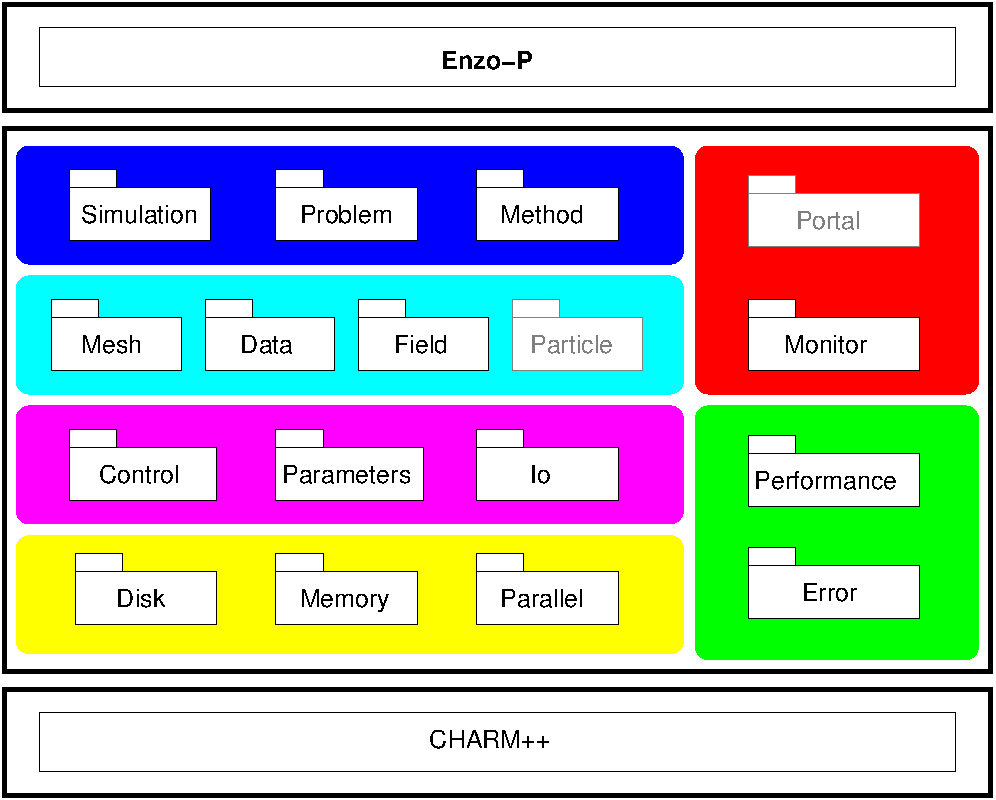
\includegraphics[width=3.0in]{components-1509.pdf}
\end{center}
\end{frame}

%----------------------------------------------------------------------

\begin{frame}[fragile] 
\secframetitle{\ssComponents}
\framesubtitle{Cello software components}
Cello's components are loosely grouped into categories
\begin{center}
\begin{minipage}{3in}
\begin{tabbing}
xxxxxxxxxxxxxxxxxxx\=\kill
\bluetext{High-level}\> \bluetext{Simulation}, \bluetext{Problem}, \bluetext{Method} \\
\cyantext{Data structures}\> \cyantext{Mesh}, \cyantext{Data}, \cyantext{Field}, \cyantext{(Particle)} \\
\magentatext{Middle-level}\> \magentatext{Control}, \magentatext{Parameters}, \magentatext{Io}  \\
\yellowtext{Hardware-interface}\> \yellowtext{Disk}, \yellowtext{Memory}, \yellowtext{Parallel} \\
\redtext{Interface}\> \redtext{Monitor}, \redtext{(Portal)}  \\
\greentext{Cross-cutting}\> \greentext{Performance}, \greentext{Error}
\end{tabbing}
\end{minipage}
\end{center}
\end{frame}

%----------------------------------------------------------------------

\begin{frame}[fragile] 
\secframetitle{\ssComponents}
\framesubtitle{\bluetext{High-level components}}
\bluebf{High-level components define the core classes in Enzo-P/Cello}

\begin{itemize}
\item \bluetext{Simulation}s define and manage computational \bluetext{Problem}s
(\bluecode{Simulation}, \bluecode{EnzoSimulation})
\item A \bluetext{Problem} defines the problem to be solved:
\begin{itemize}
\item numerical methods (\bluecode{EnzoMethodPpm}, etc.)
\item initial conditions (\bluecode{Initial})
\item boundary conditions (\bluecode{Boundary})
\item stopping criteria  (\bluecode{Stopping})
\item output (\bluecode{Output})
\item \textit{etc.}
\end{itemize}
\item A \bluetext{Method} implements a numerical method
\begin{itemize}
\item operates on block \bluetext{Data}
\end{itemize}

\end{itemize}
\end{frame}

%----------------------------------------------------------------------

\begin{frame}[fragile] 
\secframetitle{\ssComponents}
\framesubtitle{\cyantext{Data structure components}}
\cyanbf{Data structure classes define the AMR hierarchy and its data}

\begin{itemize}
\item \cyantext{Mesh} classes represent and operate on an AMR mesh (\cyancode{Hierarchy})
\item \cyantext{Data} classes store data on an AMR \textit{block} (\cyancode{Data}, \cyancode{EnzoData})
\item \cyantext{Field} classes store field data on a block
\begin{itemize}
\item \cyancode{FieldData}: field data on a block
\item \cyancode{FieldDescr}: global description of field data
\end{itemize}
\item \cyantext{Particle} classes will represent particle data on a block
\begin{itemize}
\item \cyancode{ParticleData}: particle data on a block
\item \cyancode{ParticleDescr}: global description of particle data
\end{itemize}
\end{itemize}
\end{frame}

%----------------------------------------------------------------------

\begin{frame}[fragile] 
\secframetitle{\ssComponents}
\framesubtitle{\magentatext{Middle-level components}}
\magentabf{Middle-level component interface high- and low-level classes}

\begin{itemize}
\item \magentatext{Control} handles problem evolution
\begin{itemize}
\item analagous to Enzo's \bluecode{EvolveHierarchy}, \bluecode{EvolveLevel}
\end{itemize}

\item \magentatext{Parameter} classes
\begin{itemize}
\item read parameters from a file (\magentacode{Parameters}) 
\item provide access to parameters (\magentacode{Config}, \magentacode{EnzoConfig})
\end{itemize}
\item \magentatext{Io} classes perform parallel IO
\begin{itemize}
\item \magentacode{OutputData} for writing data files
\item \magentacode{OutputImage} for writing image files
\item \magentacode{Schedule} for defining when to write files
\item \magentacode{IoHierarchy}, \magentacode{IoBlock}, \magentacode{IoFieldData}
interface data structure classes with \yellowtext{Disk} classes
\end{itemize}
\end{itemize}
%  include Control handles the time stepping of Method s to advance the
% problem forward in time, as well as sequencing adaptive mesh
% refinement data structure operations, including remeshing, scheduling
% dynamic load balancing (which will be delegated to Charm++), and
% refreshing ghost zones on Block boundaries. The Parameters component
% serves to read, store, and provide access to parameters defined in an
% input configuration file. To improve usability over Enzo,
% configuration files are more structured, and support floating-point
% and logical expressions to greatly simplify initializing problems with
% complex initial conditions. The Io component serves as a layer to
% coordinate the disk output of data structure components, such as
% Simulation Hierarchy and Field data. It calls the Disk component to
% handle actual file operations.  \end{frame}
\end{frame}

%----------------------------------------------------------------------

\begin{frame}[fragile] 
\secframetitle{\ssComponents}
\framesubtitle{\yellowtext{Hardware-interface components}}
\yellowbf{Hardware-interface components interface to system libraries}

\begin{itemize}
\item \yellowtext{Disk} classes write meta-data and data to files (\yellowcode{FileHdf5})
\item \yellowtext{Memory} tracks dynamic memory allocation
\item \yellowtext{Parallel} provides helper classes for parallelization
\begin{itemize}
\item \yellowcode{ArrayMap}: how to map chare array elements to processes
\item \yellowcode{Sync}: simple counter to ease Charm++ synchronization
\end{itemize}
\end{itemize}
% The lower-level components include Disk, Memory and Parallel. The Disk
% component implements basic disk operations, isolating the specific
% file format from the higher-level Io component. Disk currently
% supports HDF5, and we propose to support the Adaptable IO System
% (ADIOS) in the future to enhance transfer of data to and from other
% HPC software components. The Memory component controls dynamic memory
% allocation and management. Currently Memory handles allocating and
% monitoring heap memory usage; proposed functionality includes
% allocating, deallocating, and transferring data between main memory,
% hardware accelerator (GPU) memory, and many-core coprocessors
% (e.g.~the Intel Xeon Phi). As with the Disk component, this serves to
% isolate lower-level details from higher-level components. The Parallel
% component currently supplies basic access to core rank and core count,
% and is being depreciated.
\end{frame}

%----------------------------------------------------------------------

\begin{frame}[fragile] 
\secframetitle{\ssComponents}
\framesubtitle{\redtext{Interface} and \greentext{Cross-cutting} components}
\redbf{Interface components link Enzo-P / Cello with the outside world}

\begin{itemize}
\item \redtext{Monitor} keeps users informed of application status (\redcode{Monitor})
\item \redtext{(Portal)} will interface with external users / applications
\end{itemize}
\ \\
\ \\

\greenbf{Cross-cutting components are for globally-accessed classes}
\begin{itemize}
\item \greentext{Performance} measures and reports on application performance
\item \greentext{Error} provides basic error-handling support
\end{itemize}
% Interface compenents include Monitor (current) and Portal
% (proposed). The Monitor component controls the user-readable summary
% of progress to stdout, and the proposed Portal component will control
% the interaction of Enzo-P with external applications running
% concurrently, such as inline analysis or real-time visualization. One
% particular such analysis and visualization application is yt, which we
% will use to help drive the design and development of the Portal
% component.  
\end{frame}

%----------------------------------------------------------------------

%\begin{frame}[fragile] 
%\secframetitle{\ssComponents}
%\framesubtitle{: \greentext{Performance}, \greentext{Error}}
% Some Cello components can in principle be called from any software
% layer—these include Performance and Error. The Performance component
% dynamically collects performance data for the running Enzo-P
% simulation, and provides a holistic summary of performance data to the
% user, as well as to software components that can adapt to optimize
% desired performance metrics. Current metrics measured include memory
% usage (via the Memory component), and computation amount and memory
% access amount (via the Performance Application Programming Interface
% (PAPI). Future support will include metrics for monitoring parallel
% communication, dynamic load balancing, and disk usage. The Error
% component will be used to detect, evaluate, and decide what to do
% about software errors; higher-level error detection and recovery will
% be handled by Charm++, which supports both simple checkpoint to disk,
% as well as double in-memory checkpoint with automatic restart.
%\end{frame}


%    include component diagram (update from nsf proposal)
%    Go through each component and describe


%  Sequence diagram
%   Hardware components
%      Disk, Memory

% Mid-level-components

% Data structure components
%     Simulation
%     Hierarchy
%     CommBlock
%     Block
%     field\_block [field\_face]
%     [particle\_block]
%     example code

% Computational components

% Control components

% Cross-cutting components

%    Cello:     src/Cello/<component>\_<Class>.[hc]pp
%    Enzo-P:    src/Enzo/enzo\_<EnzoClass>.[hc]pp
%
%    examples
%
%    include Enzo component 
%
%    Note components are meant to be agile: can and have been redefined


% Top level components of Cello include . 
% 
% 
%Hardware-interface components
% 
%  Interface components
% 
%Cross-cutting components
% 


 % What is Enzo-P's high-level design?
%======================================================================
%\NEWSEC
%======================================================================

%\subsection{\ssClasses}

\begin{frame}[fragile,label=ss-classes] 
\secframetitle{\ssClasses}
\begin{center}
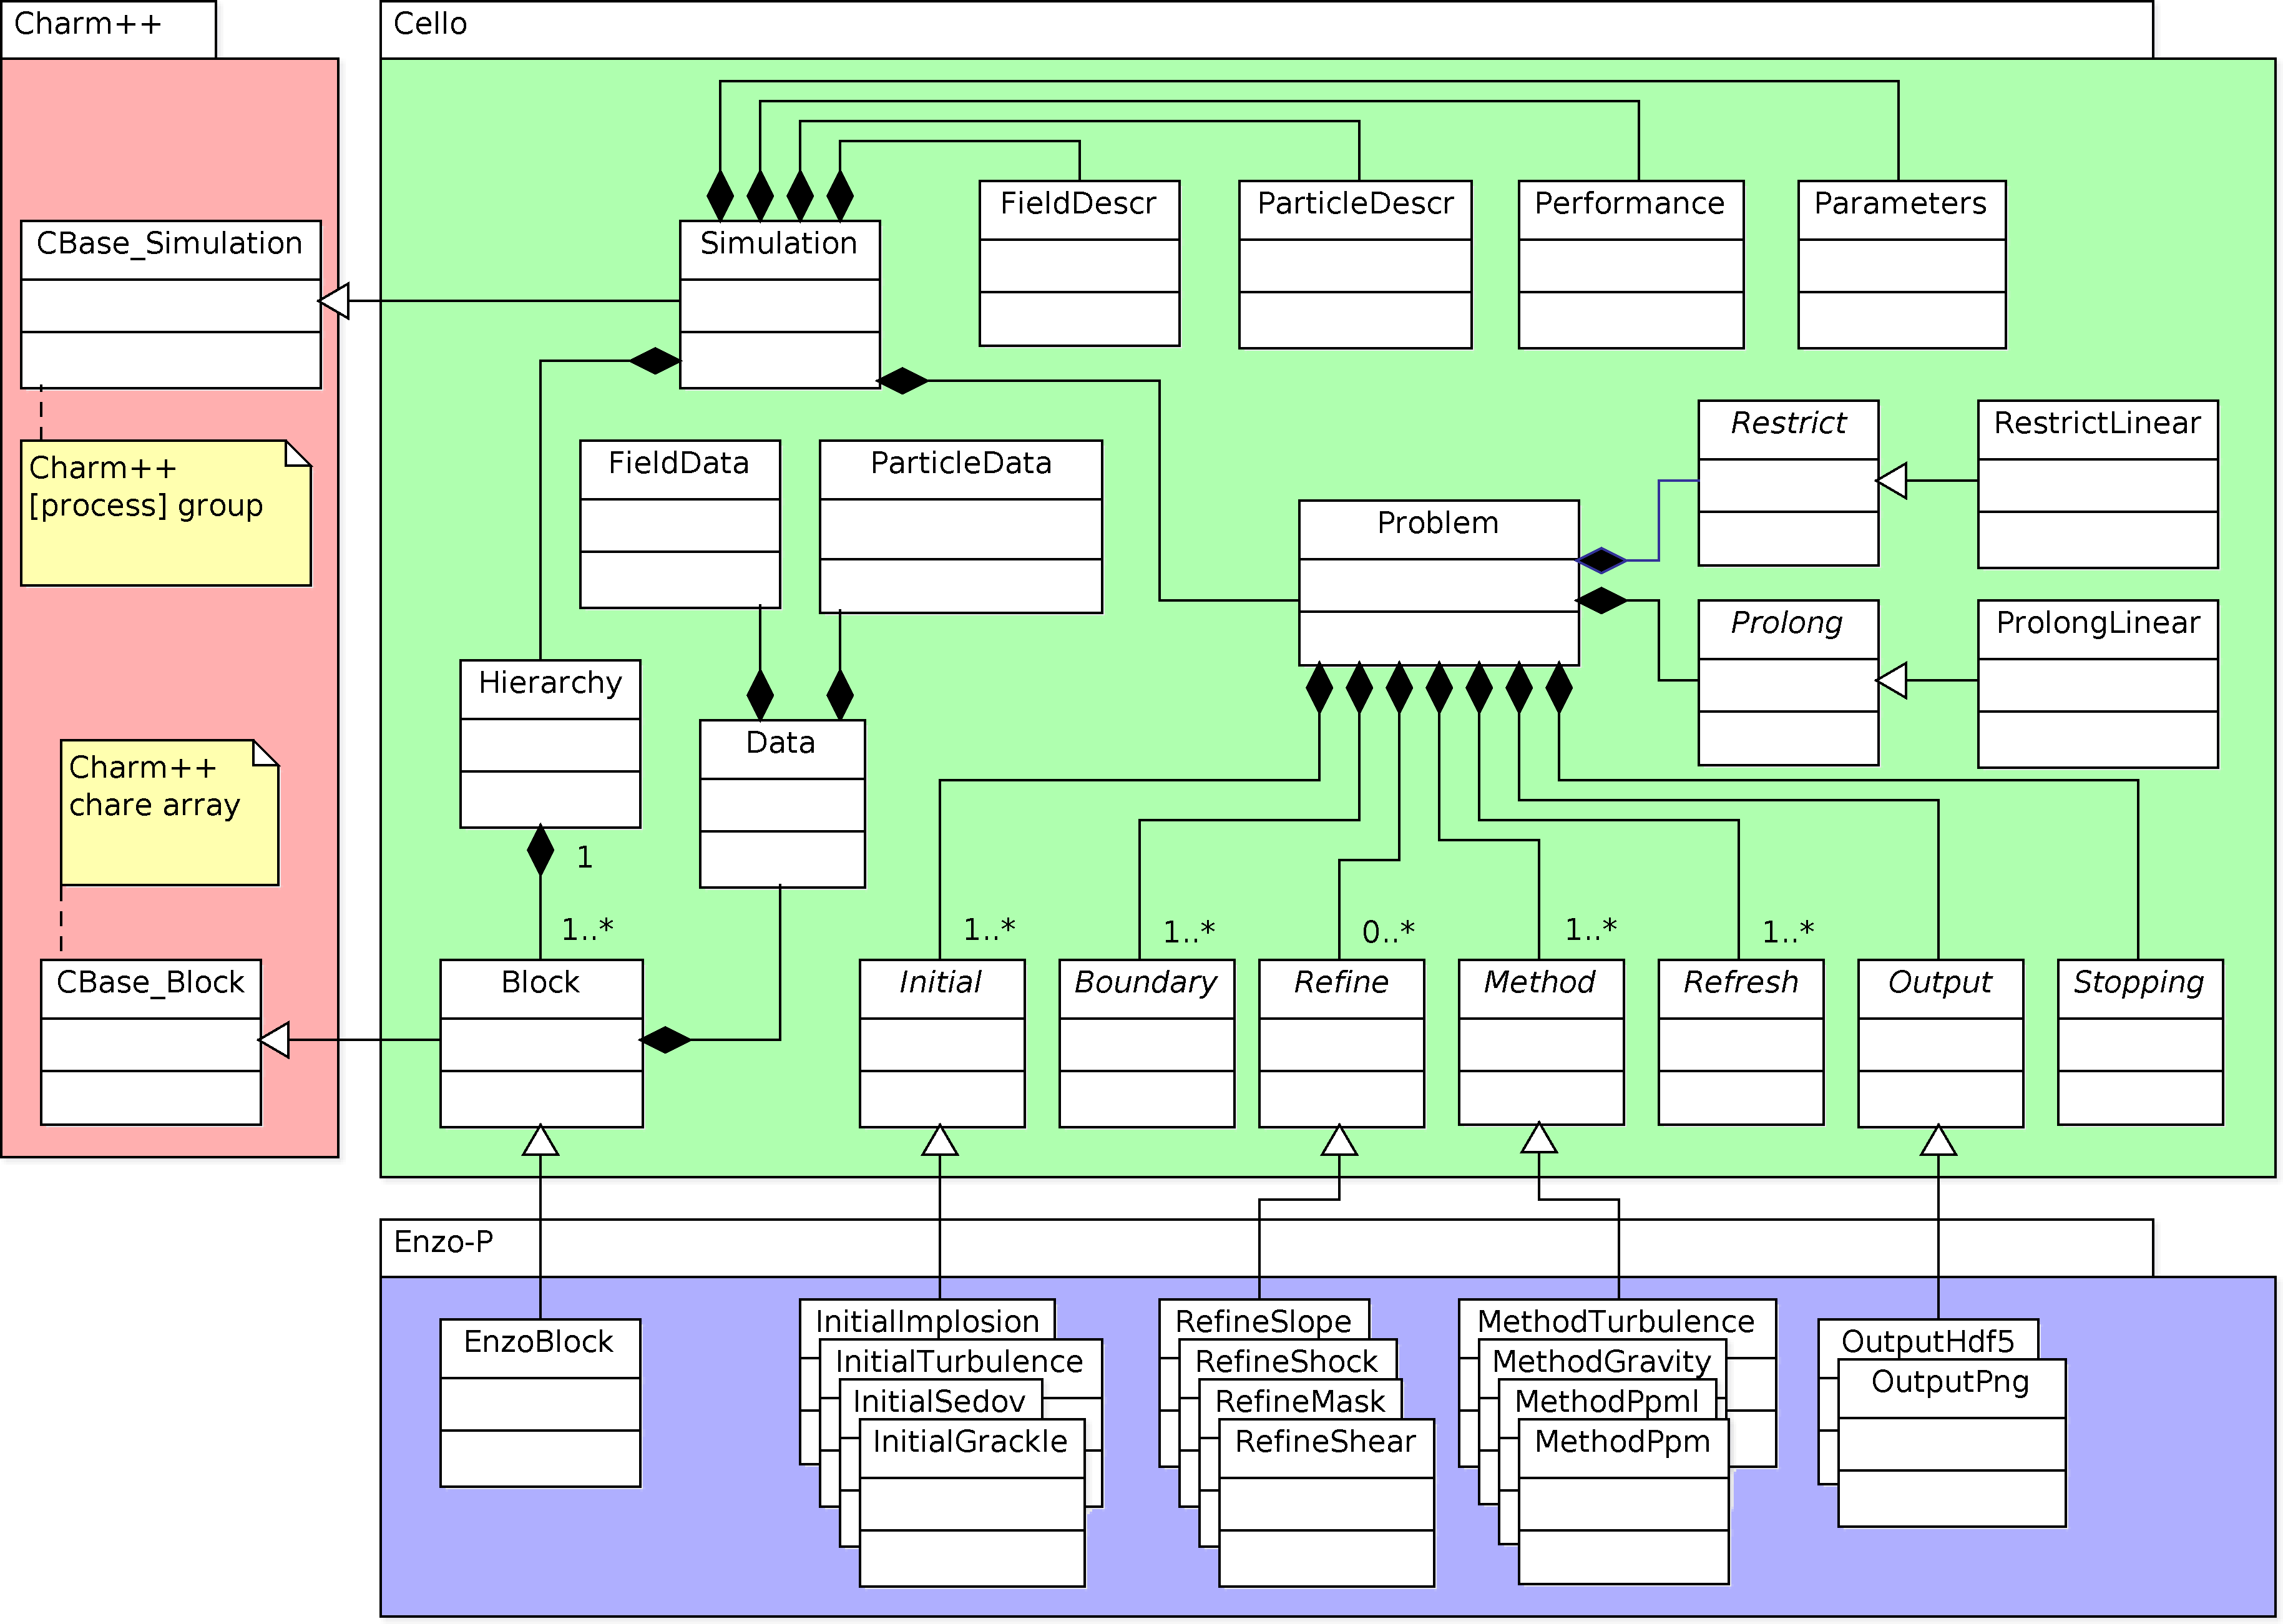
\includegraphics[width=3.5in]{ClassDiagram-color.png}
\end{center}
\end{frame}



 % How are class hierarchies represented in the code
%======================================================================
\NEWSEC
%======================================================================

\subsection{\ssClassesOrg}

\begin{frame}[fragile,label=ss-classes-org] 
\secframetitle{\ssClassesOrg}

\end{frame}

 % How are Enzo-P's classes organized?
%======================================================================
\NEWSEC
%======================================================================

\subsection{\ssProblems}

\begin{frame}[fragile,label=ss-problems] 
\secframetitle{\ssProblems}
\greenbf{Problem classes represents a numerical problem}

\begin{tabbing}
xxxx\=xxxxxxxxxxxx\=\kill
\> \greencode{Method} \>   \redit{Numerical methods} \\
\> \greencode{Initial} \>  \redit{Initial conditions} \\
\> \greencode{Boundary} \> \redit{Boundary conditions} \\
\> \greencode{Refine} \>   \redit{Mesh refinement criteria} \\
\> \greencode{Stopping} \> \redit{Stopping criteria} \\
\> \greencode{Output} \>   \redit{Disk Output} \\
\> \greencode{Prolong} \>  \redit{Interpolation scheme} \\
\> \greencode{Restrict} \> \redit{Coarsening scheme}
\end{tabbing}
\begin{itemize}
\item  Base class \greencode{Problem} initializes Cello \code{Problem} objects
\item Subclass \bluecode{EnzoProblem} initializes Enzo \code{Problem} objects
\end{itemize}
\end{frame}

 % How are problems represented in Enzo-P/Cello?
%======================================================================
\NEWSEC
%======================================================================

\subsection{\ssData}

\begin{frame}[fragile,label=ss-data] 
\secframetitle{\ssData}

\end{frame}

 % What data types are available?
%======================================================================
\NEWSEC
%======================================================================

\subsection{\ssFields}

\begin{frame}[fragile,label=ss-fields] 
\secframetitle{\ssFields}
\greenbf{Field classes represent field data on \code{Block}s}
\ \\

\begin{itemize}
\item \greencode{FieldBlock}
\begin{itemize}
\item represents state-independent (intrinsic) data
\item stored in \greencode{Block} \greencode{Data} objects
\item raw arrays
\end{itemize}
\item \greencode{FieldDescr}
\begin{itemize}
\item represents state-dependent (extrinsic) data
\item stored in \greencode{Simulation} object
\item precision, ghost depth, padding, alignment, centering
\end{itemize}
\item \greencode{Field} used to simplify using \greencode{FieldBlock} and \greencode{FieldDescr}
\end{itemize}
\end{frame}

%----------------------------------------------------------------------

\begin{frame}[fragile] 
\secframetitle{\ssFields}
\greenbf{Field class API: basic functions}
\footnotesize
\begin{semiverbatim}

   \comment{\# Return the number of fields}
   \type{int} \function{field_count} ();

   \comment{\# Return the integer handle for the named field.}
   \type{int} \function{field_id} (\variable{name});

   \comment{\# Return name of the ith field.}  
   \type{string} \function{field_name} (\variable{id});
 
\end{semiverbatim}
\end{frame}

%----------------------------------------------------------------------

\begin{frame}[fragile]
\secframetitle{\ssFields}
\greenbf{Field class API: accessing field data}
\footnotesize
\begin{semiverbatim}

   \comment{\# Return the array associated with the specified field}
   \type{char} * \function{values} (\variable{id});
   \type{char} * \function{values} (\variable{name});

   \comment{Return dimensions of fields on the data, assuming centered.}
   \keyword{void}  \function{dimensions} (\variable{id}, *\variable{mx}, *\variable{my}=\valuetext{0}, *\variable{mz}=\valuetext{0})

   \comment{\# Return size of fields on the data, assuming centered.}
   \keyword{void} \function{size} (*\variable{nx}, *\variable{ny}=\valuetext{0}, *\variable{nz}=\valuetext{0})

\end{semiverbatim}
\link{field-access}{Accessing field data is relatively easy}

\end{frame}

%----------------------------------------------------------------------

\begin{frame}[fragile]
\secframetitle{\ssFields}
\greenbf{Field class API: field characteristics}
\footnotesize
\begin{semiverbatim}

   \comment{\# Ghost depth of each field}
   \keyword{void} \function{set_ghost_depth} (\variable{id},  \variable{gx},  \variable{gy}=\valuetext{0},  \variable{gz}=\valuetext{0});
   \keyword{void} \function{ghost_depth}     (\variable{id}, *\variable{gx}, *\variable{gy}=\valuetext{0}, *\variable{gz}=\valuetext{0});

   \comment{\# Precision of each field: single, double, long double}
   \keyword{void} \function{set_precision} (\variable{id}, \variable{precision});
    \type{int} \function{precision}     (\variable{id});

   \comment{\# Cell centering of each field: -1, 0, or 1}
   \keyword{void} \function{set_centering} (\variable{id},  \variable{cx},  \variable{cy}=\valuetext{0},  \variable{cz}=\valuetext{0});
   \keyword{void} \function{centering}     (\variable{id}, *\variable{cx}, *\variable{cy}=\valuetext{0}, *\variable{cz}=\valuetext{0});

\end{semiverbatim}
\end{frame}

%----------------------------------------------------------------------

\begin{frame}[fragile]
\secframetitle{\ssFields}
\greenbf{Field class API: performance}
\footnotesize
\begin{semiverbatim}

   \comment{\# Byte alignment of field arrays in memory}
   \keyword{void} \function{set_alignment} (\variable{alignment});
    \type{int} \function{alignment} ();

   \comment{\# Byte padding between field arrays in memory}
   \keyword{void} \function{set_padding} (\variable{padding});
    \type{int} \function{padding} ();

\end{semiverbatim}
\end{frame}

%----------------------------------------------------------------------

\begin{frame}[fragile]
\secframetitle{\ssFields}
\greenbf{Field class API: fields can be associated with groups}
\footnotesize
\begin{semiverbatim}

   \comment{\# Return the Grouping object for the Fields}
   \type{Grouping} * \type{Field}::\function{groups} ();

   \comment{\# Add an item to a group. (Cello)}
   \keyword{void} \type{Grouping}::\function{add} (\variable{item}, \variable{group});
   
   \comment{\# Return whether the item is in the given Grouping.}
   \type{bool} \type{Grouping}::\function{is_in} (item, group)

   \comment{\# Return the number of items in the Grouping.}
   \type{int} \type{Grouping}::\function{size} (\variable{item})
   
   \comment{\# Return the ith Field in the Grouping.} 
   \type{string} \type{Grouping}::\function{item} (\variable{group}, \variable{i});

\end{semiverbatim}
\end{frame}

%   std::string field\_name(size\_t id) const throw(std::out\_of\_range)
% 
%   bool is\_field(const std::string \& name) const throw()
%   int field\_id(const std::string \& name) const throw()
%   Grouping * groups () 
%   void centering(int id, int * cx, int * cy = 0, int * cz = 0) const 
%   void ghosts(int id, int * gx, int * gy = 0, int * gz = 0) const 
%     throw(std::out\_of\_range)
%   int precision(int id) const throw(std::out\_of\_range)
%   int bytes\_per\_element(int id) const throw()
%   void size(int * nx, int * ny = 0, int * nz = 0) const throw()
%   void dimensions(int id\_field,int * mx, int * my = 0, int * mz = 0) const throw()
%   char * values (int id) throw (std::out\_of\_range)
%   char * unknowns ( int id) throw (std::out\_of\_range)
%   void cell\_width(double xm,   double xp,   double * hx,
% 		  double ym=0, double yp=0, double * hy=0,
% 		  double zm=0, double zp=0, double * hz=0) const throw ()
%   void clear ( float value = 0.0, 
% 	       int id\_first = -1, 
% 	       int id\_last  = -1) throw()
%   bool ghosts\_allocated() const throw ()
%   int field\_size (int id, int *nx=0, int *ny=0, int *nz=0) const throw()

%\end{frame}

 % How are fields used in the code?
%======================================================================
\NEWSEC
%======================================================================

\subsection{Particles}
% \subsection{Classes for representing particle data}

\begin{frame}[fragile,label=ss-particles] 
\secframetitle{Classes for representing particle data}
\begin{center}
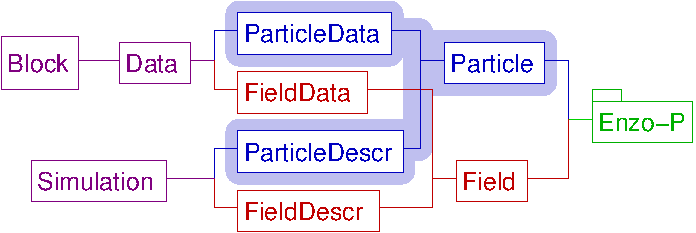
\includegraphics[width=2in]{data-classes-particle.pdf}
\end{center}

\begin{itemize}
\item \greencode{ParticleData}
\begin{itemize}
\item represents state-independent (intrinsic) data
\item associated with \greencode{Block}s (one object per mesh node)
\item stores arrays of particle data
\end{itemize}
\item \greencode{ParticleDescr}
\begin{itemize}
\item represents state-dependent (extrinsic) data
\item associated with \greencode{Simulation} objects (one per process)
\item describes how to interpret particle data (types, attributes, etc.)
\end{itemize}
\item \greencode{Particle}
\begin{itemize}
\item applications access particle data via \greencode{Particle} objects
\end{itemize}
\end{itemize}
\end{frame}

%----------------------------------------------------------------------

\begin{frame}[fragile,label=ss-particles] 
\secframetitle{How \code{Particle} objects store particle data}
\begin{minipage}{1.8in}
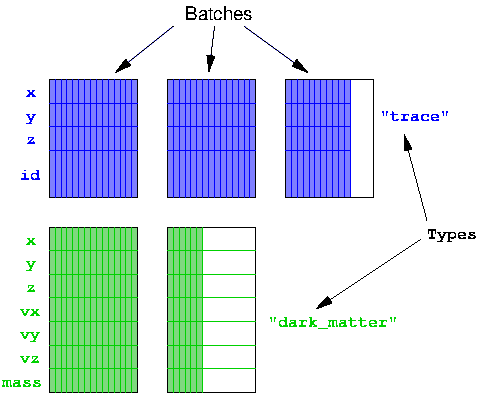
\includegraphics[width=2.0in]{particles-design.pdf} \ \\
\end{minipage} \ 
\begin{minipage}{2.5in}
\begin{itemize}
\item multiple particle \textit{types}
\item particles allocated in \textit{batches}
\begin{itemize}
\item fixed size arrays
\item fewer new/delete operations
\item efficient insert/delete operations
\item potentially useful for GPU's
\end{itemize}
\item batches store particle \textit{attributes}
\begin{itemize}
\item (position, velocity, mass, etc.)
\item 8,16,32,64-bit integers
\item 32,64,128-bit floats
\end{itemize}
\end{itemize}
\end{minipage}
\begin{itemize}
\item particle positions may be floating-point or integers
\begin{itemize}
\item floating-point for storing global positions
\item integers for \code{Block}-local coordinates
\begin{itemize}
\item solves reduced precision issue for deep hierarchies
\item less memory required for given accuracy
\end{itemize}
\end{itemize}
\end{itemize}


\end{frame}

%----------------------------------------------------------------------

\begin{frame}[fragile,label=ss-particles] 
\secframetitle{How particle data is communicated between Blocks}
\begin{itemize}
\item communication is required when particles move outside a Block 
\item this is done using a 4x4x4 array
\begin{itemize}
\item array contains pointers to ParticleData (PD) objects
\item one PD object per neighbor Block
\end{itemize}

\end{itemize}
\begin{minipage}{1.8in}
%\includegraphics<1>[width=2.0in]{particle-refresh-0.pdf}
%\includegraphics<2>[width=2.0in]{particle-refresh-1.pdf}
%\includegraphics<3>[width=2.0in]{particle-refresh-2.pdf}
%\includegraphics<4>[width=2.0in]{particle-refresh-3.pdf}
\includegraphics[width=2.0in]{particle-refresh-4.pdf}
\end{minipage} \ 
\begin{minipage}{2.7in}
\begin{itemize}
\item migrating particles are
\begin{itemize}
\item \code{scatter()}-ed to PD array objects
\item sent to associated neighbors
\item \code{gather()}-ed by neighbors
\end{itemize}
\item one sweep through particles
\item one communication step per neighbor
\item similar for refinement / coarsening
\end{itemize}
\end{minipage}
\end{frame}


 % How are particles used in the code?
%======================================================================
\NEWSEC
%======================================================================

\subsection{\ssBoundary}

\begin{frame}[fragile,label=ss-boundary] 
\secframetitle{\ssBoundary}
\greenbf{Boundary classes implement boundary conditions}
\ \\
\begin{tabbing}
xxxx\=xxxxxxxxxxxxxxxxxx\=\kill
\> \greencode{enforce()} \> \redit{Apply the boundary conditions on a} \greencode{block}
\end{tabbing}

\greentext{Current boundary conditions include}
\footnotesize
\begin{tabbing}
xxxx\=xxxxxxxxxxxxxxxxxxxxxxxxxxx\=\kill
\> \bluecode{EnzoBoundary} \> \redit{Reflecting and outflow (Greg Bryan)} \\
\> \bluecode{BoundaryPeriodic} \> \redit{Periodic} \\
\> \bluecode{BoundaryValue} \> \redit{Inflow}
\end{tabbing}
\end{frame}


 % What boundary conditions are supported?
%======================================================================
\NEWSEC
%======================================================================


\subsection{\ssInitial}

\begin{frame}[fragile,label=ss-initial] 
\secframetitle{\ssInitial}
\greenbf{Initial classes implement initial conditions}
\ \\
\begin{tabbing}
xxxx\=xxxxxxxxxxxxxxxxxxxx\=\kill
\> \greencode{enforce\_block()} \> \redit{Apply the initial conditions on a} \greencode{block}
\end{tabbing}

\greentext{Current initial conditions include}
\footnotesize
\begin{tabbing}
xxxx\=xxxxxxxxxxxxxxxxxxxxxxxxxxx\=\kill
\> \bluecode{InitialValue} \> \redit{Initialize from parameter file} \\
\> \bluecode{EnzoInitialImplosion2} \> \redit{Implosion test problem} \\
\> \bluecode{EnzoInitialSedovArray2} \> \redit{2D array of Sedov blasts  } \\
\> \bluecode{EnzoInitialSedovArray3} \> \redit{3D array of Sedov blasts} \\
\> \bluecode{EnzoInitialTurbulence} \> \redit{Turbulence initial conditions (Kritusk)  } \\
\> \bluecode{EnzoInitialGrackleTest} \> \redit{Grackle test problem (Britton) (incomplete)} \\
\> \bluecode{InitialFile} \> \redit{Initialize from a file (incomplete)  }
\end{tabbing}
\end{frame}


 % What initial conditions are supported?
%======================================================================
\NEWSEC
%======================================================================


\subsection{\ssRefine}

\begin{frame}[fragile,label=ss-refine] 
\secframetitle{\ssRefine}
\greenbf{Refine classes implement refinement criteria}
\ \\
\begin{tabbing}
xxxx\=xxxxxxxxxx\=\kill
\> \greencode{apply()} \> \redit{Apply the refinement criteria on a} \greencode{block} \\
\> \greencode{name()} \> \redit{Return the name of the criteria (e.g.~"shock")} \greencode{block}
\end{tabbing}

\greentext{Current refine conditions include}
\footnotesize
\begin{tabbing}
xxxx\=xxxxxxxxxxxxxxxxxxxxx\=\kill
\> \bluecode{RefineSlope} \> \redit{refine on relative slope} \\
% ($\lvert\frac{x_{i+1}- x_{i-1}}{2h \cdot x_i}\rvert$)
\> \bluecode{RefineDensity} \> \redit{refine on density threshold} \\
\> \bluecode{RefineMask} \> \redit{refine according to level array} \\
\> \bluecode{RefineShear} \> \redit{refine on shear} \\
\> \bluecode{EnzoRefineShock} \> \redit{refine on shocks} \\
\> \bluecode{RefineMass} \> \redit{refine on minimum mass (not implemented)}
\end{tabbing}
\end{frame}


 % What refinement criteria are supported?
%======================================================================
\NEWSEC
%======================================================================

\subsection{\ssStopping}

\begin{frame}[fragile,label=ss-stoppig] 
\secframetitle{\ssStopping}

class Stopping

\end{frame}

 % What stopping criteria are supported?
%======================================================================
\NEWSEC
%======================================================================

\subsection{\ssMethods}

\begin{frame}[fragile,label=ss-methods] 
\secframetitle{\ssMethods}
\greenbf{Method classes implement numerical methods on \code{Block}s}
\ \\
\begin{tabbing}
xxxx\=xxxxxxxxxxxxxx\=\kill
\> \greencode{compute()} \> \redit{Apply the method to a} \greencode{block} \\
\> \greencode{name()}    \> \redit{Return the method name (e.g.} \redcode{"ppm"}) \\
\> \greencode{timestep()} \> \redit{Return maximum allowed timestep}
\end{tabbing}

\greentext{Current methods include}
\footnotesize
\begin{tabbing}
xxxx\=xxxxxxxxxxxxxxxxxxxxxxxxxxxxx\=\kill
\> \bluecode{EnzoMethodPpm} \> \redit{PPM hydrodynamics (Greg Bryan et al)} \\
\> \bluecode{EnzoMethodPpml} \> \redit{PPML ideal MHD (Sergey Ustyugov)} \\
\> \bluecode{EnzoMethodHeat} \> \redit{Forward Euler heat equation } \\
\> \bluecode{EnzoMethodGravityBiCGStab} \> \redit{BiCG-STAB gravity solver (Dan Reynolds)} \\
\> \bluecode{EnzoMethodGravityCg} \> \redit{CG gravity solver } \\
\> \bluecode{EnzoMethodGravityMg0} \> \redit{MG root-grid gravity solver  (incomplete)} \\
\> \bluecode{EnzoMethodGravityMlat} \> \redit{MG gravity solver  (incomplete)} \\
\> \bluecode{EnzoMethodGrackle} \> \redit{Grackle chemistry (Britton Smith) (incomplete)} \\
\> \bluecode{EnzoMethodTurbulence} \> \redit{Turbulent mixing (Alexei Kritsuk)}
\end{tabbing}
\end{frame}


 % What numerical methods are available?
%
%======================================================================
\NEWSEC
%======================================================================

\subsection{\ssControl}

\begin{frame}[fragile,label=ss-control] 
\secframetitle{\ssControl}

\bluebf{Simulation evolution is controlled in} \bluecode{control\_charm.cpp}

\tikzstyle{decision} = [diamond, draw, fill=blue!20, 
    text width=4.5em, text badly centered, node distance=3cm, inner sep=0pt]
\tikzstyle{block} = [rectangle, draw, fill=blue!20, 
    text width=5em, text centered, rounded corners, minimum height=4em]
\tikzstyle{line} = [draw, -latex']
\tikzstyle{cloud} = [draw, ellipse,fill=red!20, node distance=3cm,
    minimum height=2em]
\ \\
\begin{tikzpicture}[node distance = 3cm, auto]
   \node [block] (init) {Initialize};
   \node [block,below of=init, node distance = 2cm] (adapt) {Adapt};
   \node [block,right of=adapt] (output) {Output};
   \node [block,right of=output] (stopping) {Stopping criteria};
   \node [block,right of=stopping] (compute) {Compute}; 
   \node [block, above of=compute, node distance = 2cm] (refresh) {Refresh};
   \node [coordinate, below of=compute, node distance = 1.5cm] (computenode) {};
   \node [coordinate, below of=adapt, node distance = 1.5cm] (adaptnode) {};

   \path [line] (init) -- (adapt);   
   \path [line] (adapt) -- (output);   
   \path [line] (output) -- (stopping);   
   \path [line] (stopping) -- (compute);   
   \path [line] (compute) -- (refresh);   
   \path [line] (refresh) -- (compute);   
%   \path [line] (compute) -- (adapt);   
 \path [line] (compute.south) -|  (computenode) -- (adaptnode) |- (adapt.south);
\end{tikzpicture}

\end{frame}

 % How are phases of the computation controlled?
%======================================================================
\NEWSEC
%======================================================================

\subsection{\ssAmr}

%----------------------------------------------------------------------

\begin{frame}[fragile,label=ss-amr] 
\secframetitle{\ssAmr}
\begin{center}
\begin{minipage}{1in}
   \includegraphics<1->[width=1in]{enzo-sedov.png}
\end{minipage} \ 
\begin{minipage}{2.5in}
\blockblue
\begin{block}<+->{\textbf{\enzo}}
Structured AMR \\
Variable shaped patches \\
Neighbors \& parent communication
  \end{block}
\end{minipage} \\
\vspace{0.1in}
\begin{minipage}{1in}
   \includegraphics<2->[width=1in]{cello-sedov.png}
\end{minipage} \ 
\begin{minipage}{2.5in}
\blockgreen
   \begin{block}<+->{\textbf{\enzopcello}}
Array of octrees \\
Fixed shaped blocks \\
neighbors only communication
   \end{block}
\end{minipage}
\end{center}

\end{frame}

%----------------------------------------------------------------------

\begin{frame}[fragile] 
\secframetitle{\ssAmr}
\blockblue
\begin{block}<+->{\textbf{\enzo\ AMR}}
\begin{center}
\begin{minipage}{2.5in}
   \includegraphics<1->[width=2.5in]{enzo-amr.pdf}
\end{minipage}
\end{center}
\end{block}
\vspace{-0.2in}
\blockgreen
\begin{block}<+->{\textbf{\cello\ AMR}}
\begin{center}
\begin{minipage}{2.5in}
   \includegraphics<2->[width=2.5in]{cello-amr.pdf}
\end{minipage}
\end{center}
\end{block}
\end{frame}

 % How does Cello implement AMR?
\input{ss-exchange} % How does Cello exchange data between blocks?
